\begin{figure}[H]
\centering
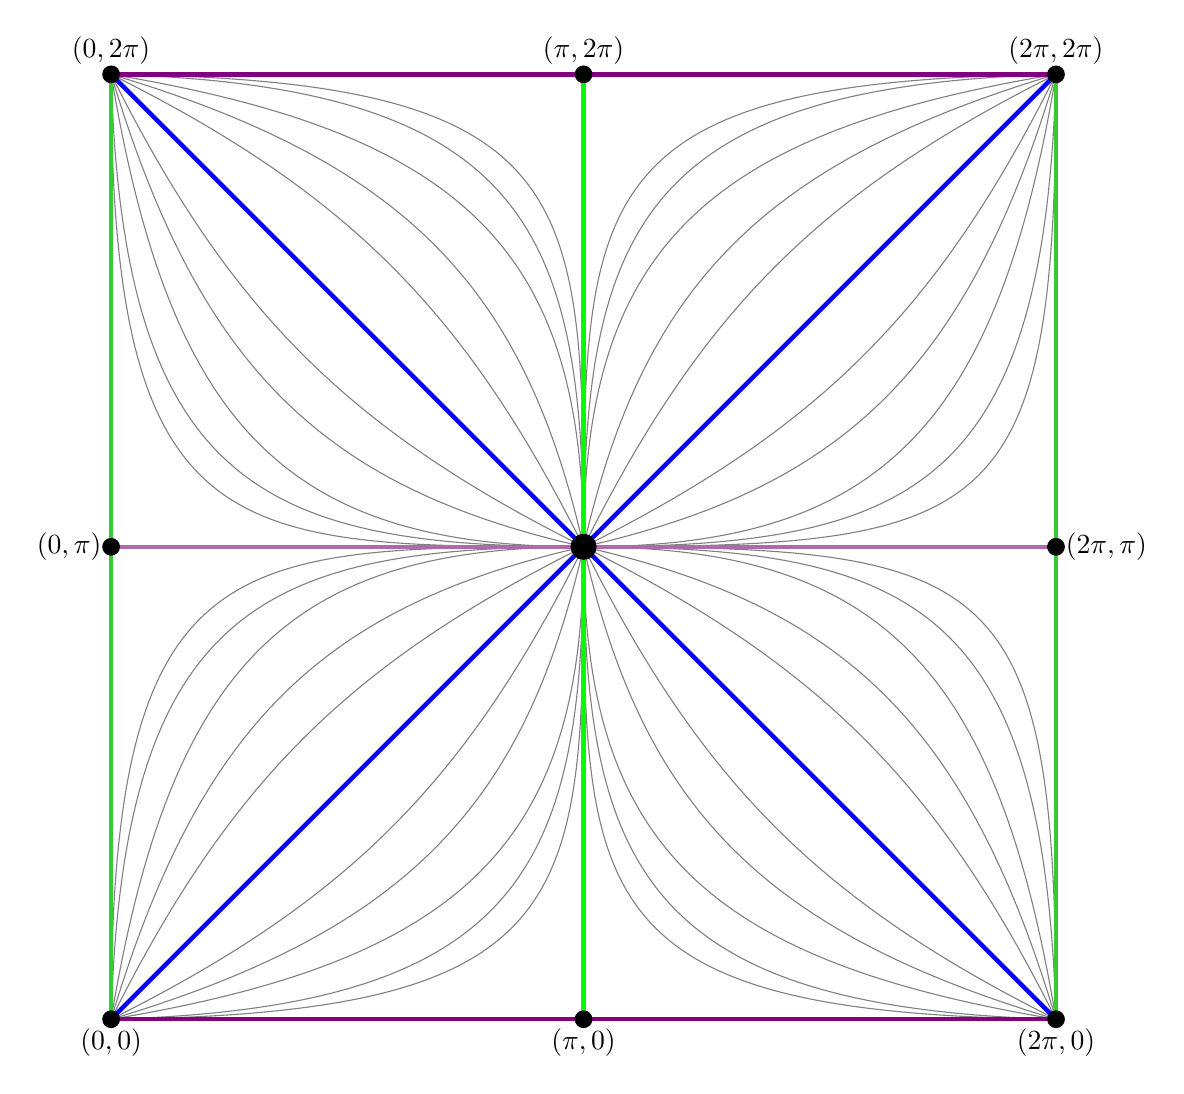
\begin{tikzpicture}[scale = 1.5]

%curves
\begin{scope}[every node/.style={sloped,allow upside down}] %top left box
    \draw[color = gray, thin]  (0,0).. controls (1,-2) and (2,-3) .. node {\midarrow}(4,-4);
    \draw[color = gray, thin]  (0,0).. controls (0.75,-2.5) and (1.8,-3.5) .. node {\midarrow}(4,-4);
    \draw[color = gray, thin]  (0,0).. controls (0.5,-3) and (1.5,-4) .. node {\midarrow}(4,-4);
    \draw[color = gray, thin] (0,0).. controls (0.1,-3.5) and (1.3,-4) .. node {\midarrow}(4,-4);
    \draw[color = gray, thin] (0,0).. controls (0,-4) and (1,-4) .. node {\midarrow}(4,-4);
    \draw[color = gray, thin]  (0,0).. controls (2,-1) and (3,-2) .. node {\midarrow}(4,-4);
    \draw[color = gray, thin]  (0,0).. controls (2.5,-0.75) and (3.5,-1.8) .. node {\midarrow}(4,-4);
    \draw[color = gray, thin]  (0,0).. controls (3,-0.5) and (4,-1.5) .. node {\midarrow}(4,-4);
    \draw[color = gray, thin] (0,0).. controls (3.5,-0.1) and (4,-1.3) .. node {\midarrow}(4,-4);
    \draw[color = gray, thin] (0,0).. controls (4,-0.05) and (4,-1) .. node {\midarrow}(4,-4);
\end{scope}

\begin{scope}[every node/.style={sloped,allow upside down}] %top right box
    \draw[color = gray, thin]  (8,0).. controls (7,-2) and (6,-3) .. node {\midarrow}(4,-4);
    \draw[color = gray, thin]  (8,0).. controls (7.25,-2.5) and (6.2,-3.5) .. node {\midarrow}(4,-4);
    \draw[color = gray, thin]  (8,0).. controls (7.5,-3) and (6.5,-4) .. node {\midarrow}(4,-4);
    \draw[color = gray, thin] (8,0).. controls (7.9,-3.5) and (6.8,-4) .. node {\midarrow}(4,-4);
    \draw[color = gray, thin] (8,0).. controls (8,-3.8) and (7.5,-4) .. node {\midarrow}(4,-4);
    \draw[color = gray, thin]  (8,0).. controls (6,-1) and (5,-2) .. node {\midarrow}(4,-4);
    \draw[color = gray, thin]  (8,0).. controls (5.5,-0.75) and (4.5,-1.8) .. node {\midarrow}(4,-4);
    \draw[color = gray, thin]  (8,0).. controls (5,-0.5) and (4,-1.5) .. node {\midarrow}(4,-4);
    \draw[color = gray, thin] (8,0).. controls (4.5,-0.1) and (4,-1.3) .. node {\midarrow}(4,-4);
    \draw[color = gray, thin] (8,0).. controls (4,-0.05) and (4,-1) .. node {\midarrow}(4,-4);    
\end{scope}

\begin{scope}[every node/.style={sloped,allow upside down}] %bottom left box
    \draw[color = gray, thin]  (0,-8).. controls (1,-6) and (2,-5) .. node {\midarrow}(4,-4);
    \draw[color = gray, thin]  (0,-8).. controls (0.75,-5.5) and (1.8,-4.5) .. node {\midarrow}(4,-4);
    \draw[color = gray, thin]  (0,-8).. controls (0.5,-5) and (1.5,-4) .. node {\midarrow}(4,-4);
    \draw[color = gray, thin] (0,-8).. controls (0.1,-4.5) and (1.3,-4) .. node {\midarrow}(4,-4);
    \draw[color = gray, thin] (0,-8).. controls (0,-4) and (1,-4) .. node {\midarrow}(4,-4);
    \draw[color = gray, thin]  (0,-8).. controls (2,-7) and (3,-6) .. node {\midarrow}(4,-4);
    \draw[color = gray, thin]  (0,-8).. controls (2.5,-7.25) and (3.5,-6.2) .. node {\midarrow}(4,-4);
    \draw[color = gray, thin]  (0,-8).. controls (3,-7.5) and (4,-6.5) .. node {\midarrow}(4,-4);
    \draw[color = gray, thin] (0,-8).. controls (3.5,-7.9) and (4,-6.7) .. node {\midarrow}(4,-4);
    \draw[color = gray, thin] (0,-8).. controls (4,-7.95) and (4,-7) .. node {\midarrow}(4,-4);
\end{scope}


\begin{scope}[every node/.style={sloped,allow upside down}] %bottom right box
    \draw[color = gray, thin]  (8,-8).. controls (6,-7) and (5,-6) .. node {\midarrow}(4,-4);
    \draw[color = gray, thin]  (8,-8).. controls (5.5,-7.25) and (4.5,-6.2) .. node {\midarrow}(4,-4);
    \draw[color = gray, thin]  (8,-8).. controls (5,-7.5) and (4,-6.5) .. node {\midarrow}(4,-4);
    \draw[color = gray, thin] (8,-8).. controls (4.5,-7.9) and (4,-6.7) .. node {\midarrow}(4,-4);
    \draw[color = gray, thin] (8,-8).. controls (4,-7.95) and (4,-7) .. node {\midarrow}(4,-4);
    \draw[color = gray, thin]  (8,-8).. controls (7,-6) and (6,-5) .. node {\midarrow}(4,-4);
    \draw[color = gray, thin]  (8,-8).. controls (7.25,-5.5) and (6.2,-4.5) .. node {\midarrow}(4,-4);
    \draw[color = gray, thin]  (8,-8).. controls (7.5,-5) and (6.5,-4) .. node {\midarrow}(4,-4);
    \draw[color = gray, thin] (8,-8).. controls (7.9,-4.5) and (6.8,-4) .. node {\midarrow}(4,-4);
    \draw[color = gray, thin] (8,0-8).. controls (8,-4.2) and (7.5,-4) .. node {\midarrow}(4,-4);
\end{scope}



%Border
\begin{scope}[every node/.style={sloped,allow upside down}]
    \draw[color = violet!100, ultra thick] (0,0) -- node {\midarrow} (4, 0); \draw[color = violet!100, ultra thick] (8, 0) -- node {\midarrow} (4, 0);
    \draw[color = green!60!gray, ultra thick] (8, 0) -- node {\midarrow} (8, -4); \draw[color = green!60!gray, ultra thick] (8, -8) -- node{\midarrow} (8, -4);
    \draw[color = violet!100, ultra thick] (0, -8) -- node {\midarrow} (4, -8); \draw[color = violet!100, ultra thick] (8, -8) -- node {\midarrow} (4, -8); 
    \draw[color = green!60!gray, ultra thick] (0, 0) -- node {\midarrow} (0,-4); \draw[color = green!60!gray, ultra thick] (0, -8) -- node {\midarrow} (0, -4);
\end{scope}

%Diagonals 
\begin{scope}[every node/.style={sloped,allow upside down}]
    \draw[color = blue!100, ultra thick] (0, 0) -- node {\midarrow} (4, -4); 
    \draw[color = blue!100, ultra thick] (8, 0) -- node {\midarrow} (4, -4); 
    \draw[color = blue!100, ultra thick] (8, -8) -- node {\midarrow} (4, -4); 
    \draw[color = blue!100, ultra thick] (0, -8) -- node {\midarrow} (4, -4);
\end{scope}

%Unstable saddle curves
\begin{scope}[every node/.style={sloped,allow upside down}]
    \draw[color = green!100, ultra thick] (4, 0) -- node {\midarrow} (4, -4);
    \draw[color = green!100, ultra thick] (4, -8) -- node {\midarrow} (4, -4);
    \draw[color = violet!60, ultra thick] (0, -4) -- node {\midarrow} (4, -4);
    \draw[color = violet!60, ultra thick] (8, -4) -- node {\midarrow} (4, -4);
\end{scope}



%Labels
\filldraw[black] (0,0) circle (2pt) node[anchor=south]{$(0, 2\pi)$};
\filldraw[black] (8, 0) circle (2pt) node[anchor=south]{$(2\pi, 2\pi)$};
\filldraw[black] (0, -8) circle (2pt) node[anchor=north]{$(0, 0)$};
\filldraw[black] (8, -8) circle (2pt) node[anchor=north]{$(2\pi, 0)$};
\filldraw[black] (4, 0) circle (2pt) node[anchor=south]{$(\pi, 2\pi)$};
\filldraw[black] (0, -4) circle (2pt) node[anchor=east]{$(0, \pi)$};
\filldraw[black] (8, -4) circle (2pt) node[anchor=west]{$(2\pi, \pi)$};
\filldraw[black] (4, -8) circle (2pt) node[anchor=north]{$(\pi, 0)$};
\filldraw[black] (4, -4) circle (3pt);

\end{tikzpicture}
\caption{Phase portrait of (\ref{eq:3}) on $[0, 2\pi]\times [0, 2\pi]$}
\label{figure1}
\end{figure}
\flushleft